%-------------------------------------------------------
% SLEPc Users Manual
%-------------------------------------------------------
\chapter{\label{cap:st}ST: Spectral Transformation}
%-------------------------------------------------------

\noindent The other main \slepc object is the Spectral Transformation (\ident{ST}), which encapsulates the functionality required for acceleration techniques based on the transformation of the spectrum. As explained in chapter \ref{cap:eps}, the implemented eigensolvers work by applying an operator to a set of vectors and this operator can adopt different forms. The \ident{ST} object handles all the different possibilities in a uniform way, so that the solver can proceed without knowing which transformation has been selected. The type of spectral transformation can be specified at run time, as well as several parameters such as the value of the shift.
	
%---------------------------------------------------
\section{General Description}

	Spectral transformations are powerful tools for manipulating the way in which eigensolvers behave when coping with a problem. The general strategy consists in transforming the original problem into a new one in which eigenvalues are mapped to a new position while eigenvectors remain unchanged. These transformations can be used with several goals in mind:
\begin{itemize}
\item Avoid convergence problems. For instance, simple methods such as the Power Iteration can fail to obtain the solution under certain conditions, and sometimes this situation  can be avoided by simply shifting the spectrum.
\item Compute internal eigenvalues. In some applications, the eigenpairs of interest are not the extreme ones (largest magnitude, smallest magnitude, rightmost, leftmost), but those contained in a certain interval or those closest to a certain value of the complex plane.
\item Accelerate convergence. Convergence properties typically depend on how close the eigenvalues are from each other. With some spectral transformations, difficult eigenvalue distributions can be remapped in a more favorable way in terms of convergence. 
\item Handle some special situations. For instance, in generalized problems when matrix $B$ is singular, it may be necessary to use a spectral transformation.
\end{itemize}
	
	\slepc separates spectral transformations from solution methods so that any combination of them can be specified by the user. To achieve this, all the eigensolvers contained in \ident{EPS} must be implemented in such a way that they are independent of which transformation has been selected by the user. That is, the solver algorithm has to work with a generic operator, whose actual form depends on the transformation used. After convergence, eigenvalues are transformed back appropriately. 

%---------------------------------------------------
\section{Basic Usage}

	The \ident{ST} module is the analogue to other \petsc{} modules such as \ident{PC}. 
	The user does not usually need to create a stand-alone \ident{ST} object explicitly. Instead, every \ident{EPS} object internally sets up an associated \ident{ST}. Therefore, the usual object management methods such as \ident{STCreate}, \ident{STDestroy}, \ident{STView}, \ident{STSetFromOptions}, are not usually called by the user.

	Although the \ident{ST} context is hidden inside the \ident{EPS} object, the user still has control over all the options, by means of the command line, or also inside the program. To allow application programmers to set any of the spectral transformation options directly within the code, the following routine is provided to extract the \ident{ST} context from the \ident{EPS} object,
	\findex{EPSGetST}
	\begin{Verbatim}[fontsize=\small]
	EPSGetST(EPS eps,ST *st);
	\end{Verbatim}
	
	After this, one is able to set any options associated to the \ident{ST} object. For example, to set the value of the shift, the following function is available
	\findex{STSetShift}
	\begin{Verbatim}[fontsize=\small]
	STSetShift(ST st,PetscScalar shift);
	\end{Verbatim}
	This can also be done with the command line option \Verb!-st_shift <shift>!. [Note: the argument \texttt{shift} is defined as a \texttt{PetscScalar}, and this means that complex shifts are not allowed unless the complex version of \slepc is used --- see section \ref{sec:complex} for a detailed discussion of this issue.]

	Other object operations are available which are not usually called by the user. The most important of such functions are \ident{STApply}, which applies the operator to a vector, \ident{STApplyB}, which applies matrix $B$ to a vector, and \ident{STSetUp} which prepares all the necessary data structures before the solution process starts. The operator refers to one of $A$, $B^{-1}\!A$, $A+\sigma I$, ...\ depending on which kind of spectral transformation is being used.
 
%---------------------------------------------------
\section{Available Transformations}

	This section describes the spectral transformations which are provided in \slepc. As in the case of eigensolvers, the spectral transformation to be used can be specified procedurally or via the command line. The application programmer can set it by means of the command
	\findex{STSetType}
	\begin{Verbatim}[fontsize=\small]
	STSetType(ST st,STType type);
	\end{Verbatim}
where \texttt{type} can be one of 
\texttt{STSHIFT},
\texttt{STSINV}, \texttt{STCAYLEY} or
\texttt{STSHELL}.
The \ident{ST} type can also be set with the options database command \Verb!-st_type! followed by the name of the method (see table \ref{tab:transforms}).

\begin{table}[t]
\centering
{\small \begin{tabular}{lllc}
                        &                   & {\footnotesize Options} &\\
Spectral Transformation & \ident{STType}    & {\footnotesize Name}    & Operator\\\hline
Shift of Origin         & \texttt{STSHIFT}  & \texttt{shift}   & $B^{-1}A+\sigma I$\\
Shift-and-invert        & \texttt{STSINV}   & \texttt{sinvert} & $(A-\sigma B)^{-1}B$\\
Cayley                  & \texttt{STCAYLEY} & \texttt{cayley}  & $(A-\sigma B)^{-1}(A+\tau B)$\\
Shell Transformation    & \texttt{STSHELL}  & \texttt{shell}   & \emph{user-defined}\\\hline
\end{tabular} }
\caption{\label{tab:transforms}Spectral transformations available in the  \ident{ST} package.}
\end{table}

	The first three spectral transformations are described in detail in the rest of this section. The last possibility, \texttt{STSHELL}, uses a specific, application-provided spectral transformation. Section \ref{sec:shell} describes how to implement one of this transformations.

	The last column of Table \ref{tab:transforms} shows a general form of the operator used in each case. This generic operator can adopt different particular forms depending on whether the eigenproblem is standard or generalized, or whether the value of the shift ($\sigma$) and antishift ($\tau$) is zero or not. All the possible combinations are illustrated in table \ref{tab:op}.
	\begin{table}
	\centering
	{\small \begin{tabular}{llcc}
	\ident{ST}     & Choice of $\sigma,\tau$ & Standard problem & Generalized problem \\\hline
	\texttt{shift}
        & $\sigma=0$     & $A$           & $B^{-1}A$          \\
	& $\sigma\not=0$ & $A+\sigma I$  & $B^{-1}A+\sigma I$ \\ \hline
	\texttt{sinvert}
        & $\sigma=0$     & $A^{-1}$      & $A^{-1}B$          \\
	& $\sigma\not=0$ & $(A-\sigma I)^{-1}$  & $(A-\sigma B)^{-1}B$ \\ \hline
	\texttt{cayley}
	& $\sigma\not=0,\tau=0$ & $(A-\sigma I)^{-1}A$  & $(A-\sigma B)^{-1}A$ \\
        & $\sigma=0,\tau\not=0$     & $I+\tau A^{-1}$      & $I+\tau A^{-1}B$ \\
	& $\sigma\not=0,\tau\not=0$ & $(A-\sigma I)^{-1}(A+\tau I)$  & $(A-\sigma B)^{-1}(A+\tau B)$ \\ \hline
	\end{tabular} }
	\caption{\label{tab:op}Operators used in each spectral transformation mode.}
	\end{table}

	The expressions shown in table \ref{tab:op} are not built explicitly. Instead, the appropriate operations are carried out when applying the operator to a certain vector. The inverses imply the solution of a linear system of equations which is managed by setting up an associated \ident{KSP} object. The user can control the behavior of this object by adjusting the appropriate options, as will be illustrated with examples in section \ref{sec:lin}.

	In the table, the value $\sigma$ represents the shift, whereas $\tau$ is called the antishift (used only in the Cayley transformation). As explained above, the shift can be specified via the \ident{STSetShift} function or in the command line. The antishift can be given in a similar way (see \ref{sec:cayley} below).

\subsection{Default Behavior}

	By default, no spectral transformation is performed. This is equivalent to a shift of origin (\texttt{STSHIFT}) with $\sigma=0$, that is, the first line of table \ref{tab:op}. The solver works with the original expressions of the eigenvalue problems,
\begin{equation}Ax=\lambda x\;\;,\end{equation}
for standard problems, and $Ax=\lambda Bx$ for generalized ones. Note that this last equation is in fact treated internally as
\begin{equation}B^{-1}Ax=\lambda x\;\;.\end{equation}
When the eigensolver in \ident{EPS} requests the application of the operator to a vector, a matrix-vector multiplication by matrix $A$ is carried out (in the standard case) or a matrix-vector multiplication by matrix $A$ followed by a linear system solve with coefficient matrix $B$ (in the generalized case). Note that in the last case, the operation will fail if matrix $B$ is singular.

\subsection{Shift of Origin}

	The purpose of this spectral transformation (\texttt{STSHIFT}) is to shift the whole spectrum by a certain quantity, $\sigma$, which is called \emph{shift of origin}. To achieve this, the solver has to work with the shifted matrix, that is, the expressions it has to cope with are
\begin{equation}(A+\sigma I)x=\theta x\;\;,\end{equation}
for standard problems, and 
\begin{equation}(B^{-1}A+\sigma I) x=\theta x\;\;,\end{equation}
for generalized ones. The important property that is used is that shifting does not alter the eigenvectors and that it does change the eigenvalues in a simple known way, it shifts them by $\sigma$. In both the standard and the generalized problems, the following relation holds 
\begin{equation}\theta=\lambda+\sigma\;\;.\end{equation}
This means that after the solution process, the value $\sigma$ has to be subtracted from the computed eigenvalues, $\theta$, in order to retrieve the solution of the original problem, $\lambda$. This is done by means of the function \ident{STBackTransform}, which does not need to be called directly by the user.

\subsection{Shift-and-invert}

	The shift-and-invert spectral transformation (\texttt{STSINV}) is used to enhance convergence of eigenvalues in the neighbourhood of a given value. In this case, the solver deals with the expressions 
\begin{equation}(A-\sigma I)^{-1}x=\theta x\;\;,\end{equation}
for standard problems, and 
\begin{equation}(A-\sigma B)^{-1}B x=\theta x\;\;,\end{equation}
for generalized ones. 
This transformation is effective for finding eigenvalues near $\sigma$ since the eigenvalues $\theta$ of the operator that are largest in magnitude correspond to the eigenvalues $\lambda$ of the original problem that are closest to the shift $\sigma$ in absolute value. Once they are found, they may be transformed back to eigenvalues of the original problem. Again, the eigenvectors remain unchanged.
In this case, the relation between the eigenvalues of both problems is
\begin{equation}\theta=1/(\lambda-\sigma)\;\;.\end{equation}
Therefore, after the solution process, the operation to be performed in function \ident{STBackTransform} is $\lambda=\sigma+1/\theta$ for each of the computed eigenvalues.

\subsection{Cayley}
\label{sec:cayley}

	The generalized Cayley transform (\texttt{STCAYLEY}) is defined from the expressions
\begin{equation}(A-\sigma I)^{-1}(A+\tau I)x=\theta x\;\;,\end{equation}
for standard problems, and 
\begin{equation}(A-\sigma B)^{-1}(A+\tau B)x=\theta x\;\;,\end{equation}
for generalized ones. Sometimes, the term Cayley transform is applied for the particular case in which $\tau=\sigma$. This is the default if $\tau$ is not given a value explicitly. The value of $\tau$ (the anti-shift) can be set with the following function
	\findex{STCayleySetAntishift}
	\begin{Verbatim}[fontsize=\small]
	STCayleySetAntishift(ST st,PetscScalar tau);
	\end{Verbatim}
or in the command line with \Verb!-st_antishift!.

This transformation is mathematically equivalent to shift-and-invert and, therefore, it is effective for finding eigenvalues near $\sigma$ as well. However, in some situations it is numerically advantatgeous with respect to shift-and-invert (see \citep[\S 11.2]{Bai:2000:TSA}).

In this case, the relation between the eigenvalues of both problems is
\begin{equation}\theta=(\lambda+\tau)/(\lambda-\sigma)\;\;.\end{equation}
Therefore, after the solution process, the operation to be performed in function \ident{STBackTransform} is $\lambda=(\theta\sigma+\tau)/(\theta-1)$ for each of the computed eigenvalues.


%---------------------------------------------------
\section{Advanced Usage}

Using the \ident{ST} object is very straightforward. However, when using spectral transformations many things are happening behind the scenes, mainly the solution of linear systems of equations. The user must be aware of what is going on in each case, so that it is possible to guide the solution process to the most beneficial way. This section describes several advanced aspects which can have a considerable impact on efficiency.

\subsection{Solution of Linear Systems}
\label{sec:lin}

	In many of the cases shown in table \ref{tab:op}, the operator contains an inverted matrix which means that a linear system of equations must be solved whenever the application of the operator to a vector is required. These cases are handled internally by means of a \ident{KSP} object.

	In the simplest case, a generalized problem is to be solved with a zero shift. A sample command line could be
\begin{Verbatim}[fontsize=\small]
	$ program -eps_type subspace -eps_tol 1e-6 -eps_monitor
\end{Verbatim}
In this case, assuming that the program solves a generalized problem, the \ident{ST} object associated to the \ident{EPS} solver creates a \ident{KSP} object whose coefficient matrix is $B$. This \ident{KSP} object will be set with the default values, that is, GMRES with ILU preconditioning (see the \petsc{} documentation for details).

	The default values corresponding to the \ident{KSP} object can be modified via the command line. For instance,
\begin{Verbatim}[fontsize=\small]
	$ program -eps_type subspace -eps_tol 1e-6 -eps_monitor
	          -st_ksp_type cg -st_pc_type jacobi -st_ksp_rtol 1e-5
\end{Verbatim}
specifies some additional options for the solution of this linear system. In particular, this example selects the CG solver with Jacobi preconditioning and a relative tolerance of $10^{-5}$. The \Verb!-st_! prefix signifies that the option corresponds to the linear system within \ident{ST}.

	If an iterative method is used for the linear system solves, usually a slightly more stringent tolerance must be required of the linear solves relative to the desired accuracy of the eigenvalue calculation. It is also possible to select any of the direct linear solvers available in \petsc. In this case, the factorization is only carried out at the beginning of the eigenvalue calculation and this cost is amortized in each subsequent application of the operator. This is also the case for iterative methods with preconditioners with high-cost set-up such as ILU.

	The application programmer is able to set the desired linear systems solver options also from within the code. In order to do this, first the context of the \ident{KSP} object must be retrieved with the following function
	\findex{STGetKSP}
	\begin{Verbatim}[fontsize=\small]
	STGetKSP(ST st,KSP *ksp);
	\end{Verbatim}
	
	The above functionality is also applicable to the other spectral transformations. In this other example, the spectrum is shifted by $\sigma=0.5$ and several options are specified for the linear systems
\begin{Verbatim}[fontsize=\small]
	$ program -st_type shift -st_shift 0.5 -st_ksp_type cgs 
		  -st_pc_ilu_levels 1
\end{Verbatim}

	Similarly, for the shift-and-invert technique with $\sigma=10$:
\begin{Verbatim}[fontsize=\small]
	$ program -st_type sinvert -st_shift 10 -st_pc_type jacobi
\end{Verbatim}
	The shift-and-invert and Cayley transformations deserve special consideration. In these cases, the coefficient matrix is not a simple matrix but an expression which can be explicitly constructed or not, depending on the user's choice. This issue is examined in detail next.

\subsection{Explicit Computation of Coefficient Matrix}
\label{sec:explicit}

	Three possibilities can be distinguished regarding the form of the coefficient matrix of the linear systems of equations associated to the different spectral transformations. The possible coefficient matrices are:
	\begin{itemize}
	\item Simple: $B$.
	\item Shifted: $A-\sigma I$.
	\item Axpy: $A-\sigma B$.
	\end{itemize}
	The first case has already been described and presents no difficulty. In the other two cases, there are three possible approaches:
	\begin{description}
	\item[``\Verb!shell!''] To work with the corresponding expression without forming the matrix explicitly. This is achieved by internally setting a matrix-free matrix with \ident{MatCreateShell}.
	\item[``\Verb!inplace!''] To build the coefficient matrix explicitly. This is done by means of a \ident{MatShift} or a \ident{MatAXPY} operation, which overwrites matrix $A$ with the corresponding expression. This alteration of matrix $A$ is reversed after the eigensolution process has finished.
	\item[``\Verb!copy!''] To build the matrix explicitly, as in the previous option, but using a working copy of the matrix, that is, without modifying the original matrix $A$. 
	\end{description}
	The default behavior is to build the coefficient matrix explicitly in a copy of $A$ (option ``\Verb!copy!''). The user can change this as in the following example
\begin{Verbatim}[fontsize=\small]
	$ program -st_type sinvert -st_shift 10 -st_pc_type jacobi
		  -st_matmode shell
\end{Verbatim}
	As always, the procedural equivalent is also available for specifying this option in the code of the program:
	\findex{STSetMatMode}
	\begin{Verbatim}[fontsize=\small]
	STSetMatMode(ST st,STMatMode mode);
	\end{Verbatim}

	The user must consider which approach is the most appropriate for the particular application. The different options have advantatges and drawbacks. The first approach is the simplest one but severely restricts the number of possibilities available for solving the system, in particular most of the \petsc{} preconditioners would not be available, including direct methods. The only preconditioners that can be used in this case are Jacobi (only if matrices $A$ and $B$ have the operation \ident{MATOP\_GET\_DIAGONAL}) or a user-defined one.
	
	The second approach (``\Verb!inplace!'') can be much faster, specially in the generalized case. A more important advantage of this approach is that, in this case, the linear system solver can be combined with any of the preconditioners available in \petsc, including those which need to access internal matrix data-structures such as ILU. The main drawback is that, in the generalized problem, this approach probably makes sense only in the case that $A$ and $B$ have the same sparse pattern, because otherwise the function \ident{MatAXPY} can be very inefficient. 
If the user knows that the pattern is the same (or a subset), then this can be specified with the function
	\findex{STSetMatStructure}
	\begin{Verbatim}[fontsize=\small]
	STSetMatStructure(ST st,MatStructure str);
	\end{Verbatim}
	
	Note that when the value of the shift $\sigma$ is very close to an eigenvalue, then the linear system will be ill-conditioned and using iterative methods may be problematic. On the other hand, in symmetric definite problems, the coefficient matrix will be indefinite whenever $\sigma$ is a point in the interior of the spectrum and in that case it is not possible to use a symmetric definite factorization (\texttt{cholesky} or \texttt{icc}).

	The third approach (``\Verb!copy!'') uses more memory but avoids a potential problem that could appear in the ``\Verb!inplace!'' approach: the recovered matrix might be slightly different from the original one (due to roundoff).

\subsection{Shell Transformations}
\label{sec:shell}

	The \ident{ST} package allows the user to define new spectral transformations by means of the \texttt{shell} type, in a similar way as \emph{shell} preconditioners or \emph{shell} matrices. This tool is intended for simple spectral transformations. For more sophisticated transformations, the user should register a new \ident{ST} type (see section \ref{sec:extend} for details).

	At least, user-defined spectral transformations have to define how the operator is to be applied to a vector. Optionally, it can also specify the way in which computed eigenvalues must be transformed back to the solution of the original eigenproblem. An example program is provided in the \slepc distribution in order to illustrate the use of shell transformations.

	The function
	\findex{STShellSetApply}
	\begin{Verbatim}[fontsize=\small]
      STShellSetApply(ST,int(*)(void*,Vec,Vec),void*);
	\end{Verbatim}
has to be invoked after the creation of the \ident{ST} object in order to provide a routine that applies the operator to a vector. And the function
	\findex{STShellSetBackTransform}
	\begin{Verbatim}[fontsize=\small]
      STShellSetBackTransform(ST,int(*)(void*,PetscScalar*,PetscScalar*));
	\end{Verbatim}
can be used optionally to specify the routine for the back-transformation of eigenvalues. The two functions provided by the user receive a pointer to a user-defined context which can contain any useful information. This context must be passed as the last argument in the call to \ident{STShellSetApply}.

	Finally, the application programmer can use the following function
	\findex{STShellSetName}
	\begin{Verbatim}[fontsize=\small]
      STShellSetName(ST,char*);
	\end{Verbatim}
to specify a name for the new shell transformation in order to identify it in the program's output (\ident{STView}).

\subsection{Preserving the Symmetry}
\label{sec:symm}

	As mentioned in section \ref{sec:defprob}, some eigensolvers can exploit symmetry and compute a solution for Hermitian problems with less storage and/or computational cost than other methods. Also, symmetric solvers are typically more accurate. However, in the case of generalized eigenvalue problems in which both $A$ and $B$ are symmetric, we have that due to the spectral transformation, symmetry is lost because none of the operators $B^{-1}\!A+\sigma I$, $(A-\sigma B)^{-1}B$ or $(A-\sigma B)^{-1}(A+\tau B)$ is symmetric (the same applies in the Hermitian case for complex matrices).

	The solution proposed in \slepc is based on selecting different kinds of inner products. Currently, we have the following choice of inner products:
  \begin{itemize}
    \item Standard Hermitian inner product: $\langle x,y\rangle=x^Hy$
    \item $B$-inner product: $\langle x,y\rangle_B=x^H\!B\,y$
  \end{itemize}

	The second one will be used for preserving the symmetry in symmetric definite generalized problems. Note that $\langle x,y\rangle_B$ is a genuine inner product only if $B$ is symmetric positive definite. 

	$\R^n$ with $\langle x,y\rangle_B$ is isomorphic to the Euclidean $n$-space $\R^n$ with the standard Hermitian inner product. This means that if we use $\langle x,y\rangle_B$ instead of the standard inner product, we are just changing the way lengths and angles are measured, but otherwise all the algebraic properties are maintained and therefore algorithms remain correct. What is interesting to observe is that $B^{-1}\!A$ is auto-adjoint with respect to $\langle x,y\rangle_B$, and similarly with the rest of spectral transformations.

\begin{figure}[t]
  \begin{center}
    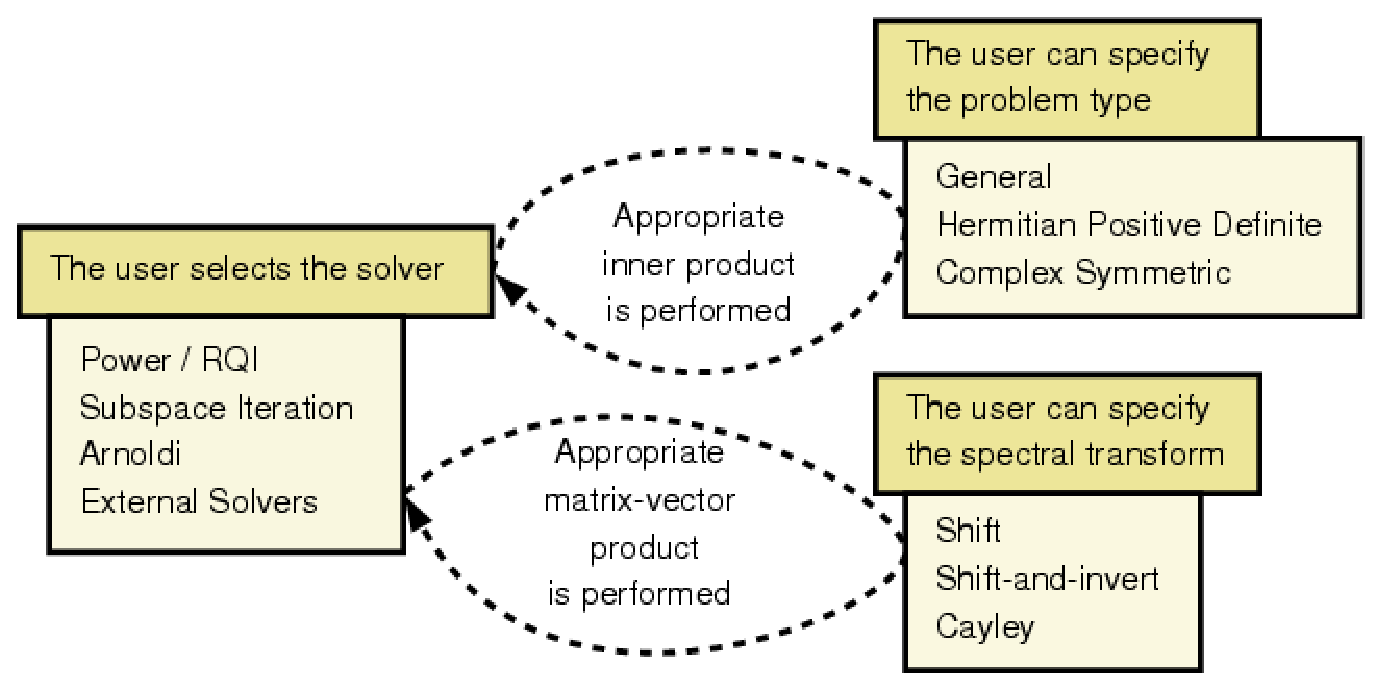
\includegraphics[width=10cm]{solvers}
  \end{center}
\caption{\label{fig:abstr}Abstraction used by \slepc solvers.}
\end{figure}

	Internally, \slepc operates with the abstraction illustrated in figure \ref{fig:abstr}. The operations indicated by dashed arrows are implemented as virtual functions: \ident{STInnerProduct} and \ident{STApply}. From the user point of view, all the above explanation is transparent. The only thing he/she has to care about is to set the problem type appropriately with \ident{EPSSetProblemType} (see section \ref{sec:defprob}).



